\documentclass[letterpaper]{article}

\usepackage{natbib,alifeconf}  %% The order is important


% *****************
%  Requirements:
% *****************
%
% - All pages sized consistently at 8.5 x 11 inches (US letter size).
% - PDF length <= 8 pages for full papers, <=2 pages for extended
%    abstracts.
% - Abstract length <= 250 words.
% - No visible crop marks.
% - Images at no greater than 300 dpi, scaled at 100%.
% - Embedded open type fonts only.
% - All layers flattened.
% - No attachments.
% - All desired links active in the files.

% Note that the PDF file must not exceed 5 MB if it is to be indexed
% by Google Scholar. Additional information about Google Scholar
% can be found here:
% http://www.google.com/intl/en/scholar/inclusion.html.


% If your system does not generate letter format documents by default,
% you can use the following workflow:
% latex example
% bibtex example
% latex example ; latex example
% dvips -o example.ps -t letterSize example.dvi
% ps2pdf example.ps example.pdf


% For pdflatex users:
% The alifeconf style file loads the "graphicx" package, and
% this may lead some users of pdflatex to experience problems.
% These can be fixed by editing the alifeconf.sty file to specify:
% \usepackage[pdftex]{graphicx}
%   instead of
% \usepackage{graphicx}.
% The PDF output generated by pdflatex should match the required
% specifications and obviously the dvips and ps2pdf steps become
% unnecessary.


% Note:  Some laser printers have a serious problem printing TeX
% output. The use of ps type I fonts should avoid this problem.


\title{Something about lineage metrics}
%\author{Chris Adami$^{1}$, Ryoichi Seki$^{1,2}$ \and Robel Yirdaw$^2$ \\
%\mbox{}\\
%$^1$California Institute of Technology, Pasadena, CA 91125 \\
%$^2$California State University, Northridge, CA 91330 \\
%adami@caltech.edu} % email of corresponding author

% For several authors from the same institution use the same number to
% refer to one address.
%
% If the names do not fit well on one line use
%         Author 1, Author 2 ... \\ {\Large\bf Author n} ...\\ ...
%
% If the title and author information do not fit in the area
% allocated, place \setlength\titlebox{<new height>} after the
% \documentclass line where <new height> is 2.25in



\begin{document}
\maketitle

\begin{abstract}

\end{abstract}

\section{Introduction}

Evolution is an emergent effect of events (\textit{e.g.} replication, variation, and competition) that occur on a much finer-grained temporal scale. While this is a large part of why it is so fascinating, it also presents challenges to studying the short-term mechanisms that govern long-term results. In computational evolutionary systems, we theoretically have adequate data to untangle these mechanisms. In practice, though, gathering appropriate data to do so can be challenging. Moreover, because of the vast difference between the scales that the causes and effects occur on, the quantity of such data can be overwhelming. Both of these problems can be mitigated with a standardized set of diagnostic summary metrics that paint a picture of shorter-term evolutionary dynamics within a population. Here, we  introduce a suite of such metrics and provide an intuition for what they can tell us about evolution.
% We test our intuitions on a set of two-dimensional, real-valued optimization problems under a range of mutation rates and selection strengths. 

% Talk about abstract idea of a lineage being a sequence of states
% A lineage can be operationally defined as a sequence of states
% talk about different things those states could be

%  Talk about metrics being a useful concept for abstracting sequence of states (because doing stats on sequences of states is hard)

%Lit review - people have made pictures but it's hard to draw abstract large-scale inferences from them

% Introduce metrics

%For the most part, the metrics we propose here will center around the evolutionary history of lineages in the population.

% @AML: Currently taking a crack at this bit of the intro (introducing lineages, etc) on paper at the moment! 
A lineage describes a continuous line of descent, linking ancestors and their descendants. A complete lineage can provide a post-hoc, step-by-step guide to the evolution of an extant organism where each step involves replication and inherited variation. Indeed, lineage analyses are a powerful tool for disentangling the evolution of complexity in both natural and digital systems; digital systems, however, allow for fine-grained lineage tracking at resolutions that are impossible in modern web lab experiments


% Something about: we often look at fitness over a lineage (i.e. fitness over time), we can look at other things... 


\section{Metrics}

\subsection{Lineage Length}
\subsection{Mutation Accumulation} 
% Count/Magnitude (by type, aggregated etc
\subsection{Phenotypic Volatility}
% Useful things that this metric could identify:
% - Mutational bet hedging (h
% - Plasticity (high volatility)
% - Neutral landscapes (expect low volatility)

\subsection{Summary statistics}

\section{Test Problems}
To understand the metrics defined above, the test problems used need to be well understood and studied. The benchmark functions from [URL OR TITLE?] meet both of these requirements and allow us to visualize the actual fitness landscape, due to the low dimensionality of the problems. For each problem, the X and Y coordinates offered by a given organism are translated by the function into a fitness value. We chose a diverse subset of these functions (Himmelblau, Shubert, Composition Function 2, and Six-Humped Camel Back) as our test problems in order to gain a broad understanding of our metrics.


\section{Data Analysis}

% Trim dramatically
%Evolutionary biologists often accuse each other of making up "just-so" stories - post-hoc explanations for how an observed trait or pattern could have evolved. The problem with these stories is that, in biology, there is often no way to verify that they reflect what happened in biology. Due to evolution's stochastic nature, it is easy to come up with possible ways that something could have happened once, regardless of how repeatable they are. Theoretically, we should easily be able to avoid this problem in computational evolution by carefully checking the underlying assumptions behind our hypothesized explanation.  All too often, however, we fail to drill down to the true underlying mechanism behind an observed effect.

%The metrics we propose here can help provide a check on this behavior, by making information about underlying evolutionary dynamics more readily accessible. They can only have that effect, however, if we completely understand what they are telling us about the way populations under different conditions are traversing different fitness landscapes. In order for these metrics to be useful for diagnosing the behavior of an evolving population, we need to establish ground truth for what underlying evolutionary dynamics are implied by different values of the metrics. For the purposes of building this intuition on a solid foundation, we wanted to be able to visualize the full evolutionary history of each population as it traversed the fitness landscape.

%To this end, we chose problems for which we could perfectly visualize the fitness landscape, and kept track of the complete evolutionary history of all members of the population. With these data, we were able to overlay successful lineages on top of the fitness landscape. Visualizing all lineages in each experimental condition in this way gave us an efficient check on our understanding of the underlying evolutionary dynamics in that condition. 

Displaying the complete history of an evolving population on a three-dimensional fitness landscape entails incorporating a large quantity of information into a limited space. When projected onto two dimensions, lineages can obscure parts of the fitness landscape (and each other). To mitigate this problem, we built the visualization using the A-Frame Framework. A-Frame supports building three dimensional scenes and rendering them to a variety of platforms. In the simplest case, the visualization is rendered in WebGL, allowing it to be viewed in a standard web browser. Mouse interactions such as rotation make it possible to view the visualization from all angles, and WebGL's use of the graphics card allows it to render data-rich visualizations. 

A-Frame also supports rendering the page with WebVR, allowing it to be viewed using various virtual reality headsets. These platforms allow the user to explore the data in a truly three-dimensional environment. Different headsets support different amounts of interaction. For the data interpretation in this paper, we used an Oculus Rift to provide us with fine-grained control of which part of the visualization we were looking at.


\section{Results and Discussion}
% Changing mutation: here's what happens when we change mutation on each problem
\begin{figure}
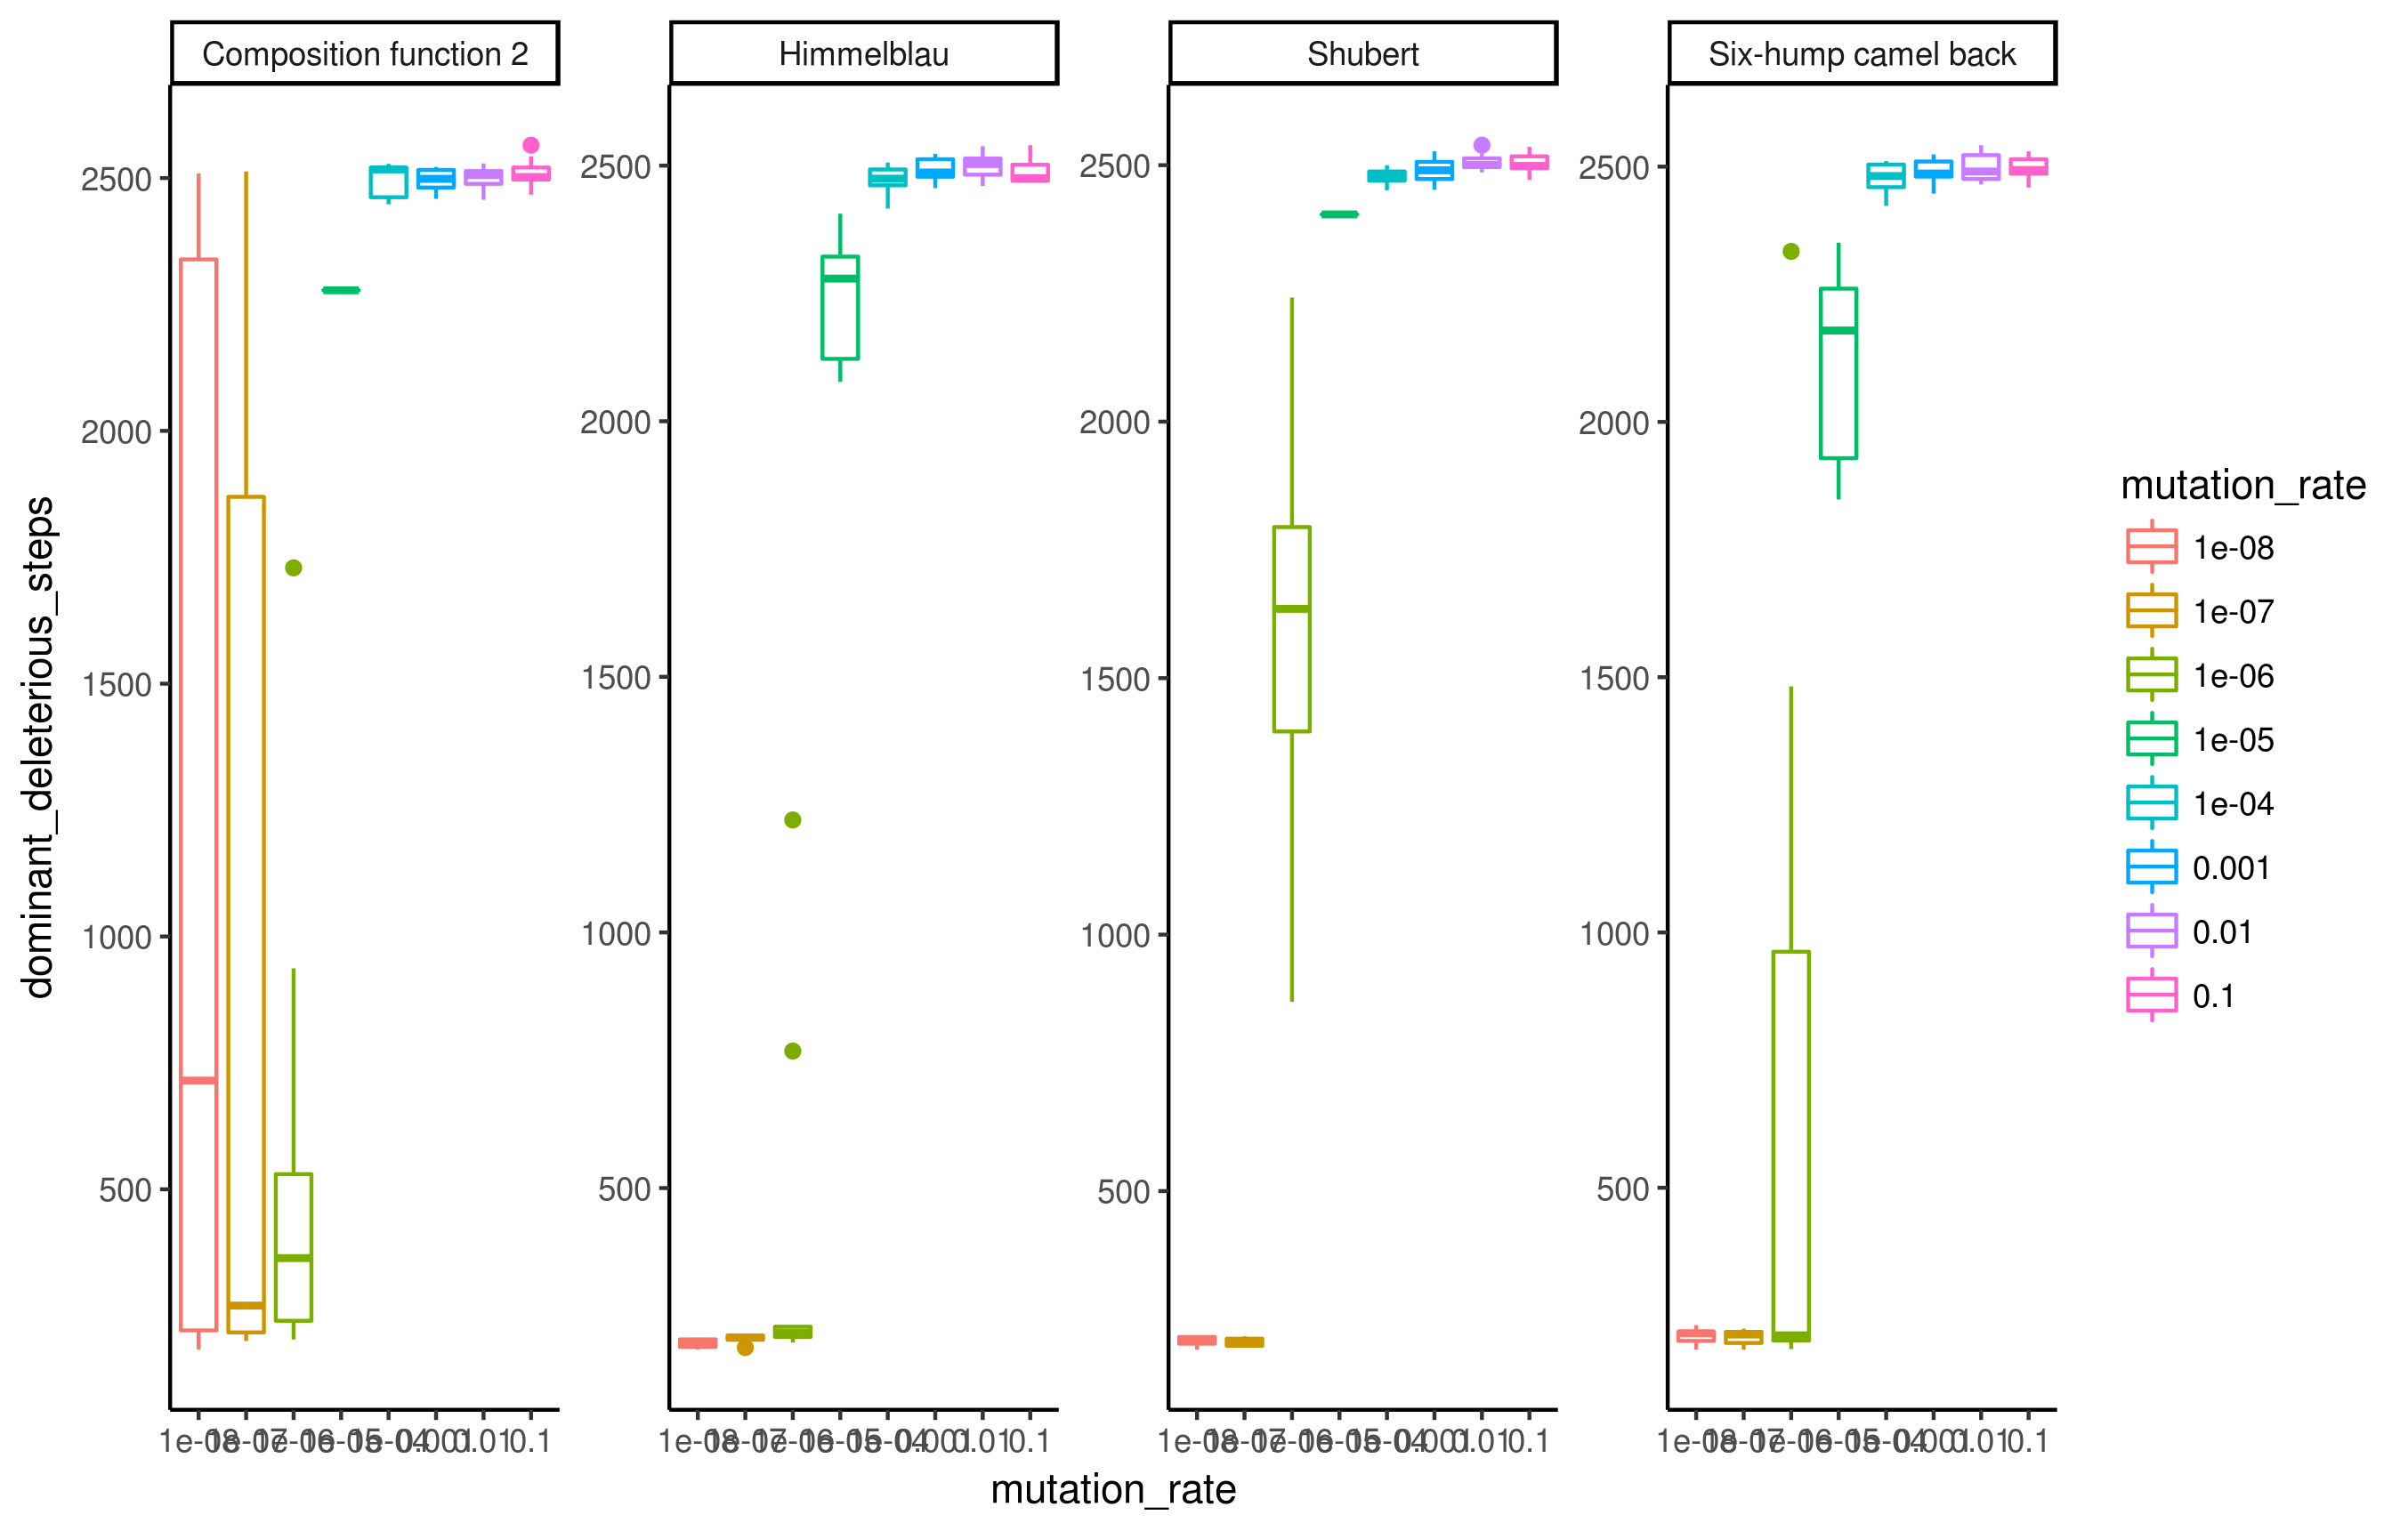
\includegraphics[width=3.5in]{figs/dom_deleterious_mutation_rate.png}
\end{figure}

% - Metric 1
% Problem 1
% Problem 2
% Problem 3
% Problem 4
% - Metric 2
% ... 

% Changing selection
% - Metric 1
% Problem 1
% Problem 2
% Problem 3
% Problem 4
% - Metric 2

\section{Conclusions}

\section{Acknowledgements}


\footnotesize
\bibliographystyle{apalike}
\bibliography{example} % replace by the name of your .bib file


% \section{Text Bank Because I'm not totally sure where things should go}
% % Some gibberish on lineages
% A lineage describes a chain of ancestors and their descendants where links in the chain are (typically) connected via parent-offspring relationships. In nature, every extant individual has a unique lineage that can be traced back to a single common ancestor. Depending on the modes of replication and variation employed along the lineage (\textit{e.g.} sexual reproduction, horizontal gene transfer), a lineage can be more or less challenging to disentangle. 
% % something something something, we focus on asexual populations w/no HGT because easy starting place. 

% % Some gibberish on how we can represent lineages as sequences of states
% Lineages can be imagined as a sequence of states where each state represents an individual. We can characterize each of these states: a phenotype, a genotype, a set of mutations (which may be empty) that differentiate genotype from parent genotype, time of birth/death, etc. 
% Given sequences, can apply diagnostic metrics...

% % Some gibberish on abstractions over the sequences of states
% We can start to make abstractions: state = genotype, state = phenotype, state = location in environment.
% Lineage length is measured over these abstractions:
% %- Length in number of individuals 
% %- Length in number of genotypes
% %- Length in number of phenotypes



\end{document}
